\chapter{Scramble architecture}
\label{ch:Scramble architecture}

Scramble is a tool to realize scalability with hierarchical orchestration. While the higher level orchestrator (Parent MANO) still controls the life-cycle of the deployed network services, scramble acts as a bridge between parent MANO and lower level orchestrator (child MANO) thus allowing interconnection between different MANO's to provide end-to-end service.  
 
\section{Architecture}
\paragraph{}
The services of scramble resides as a plugin within MANO frameworks such as SOTANA/Pishahang and Open Source MANO (OSM) and enables cross MANO communication. Service requests received by the higher level MANOs in the hierarchy can be routed to lower level MANOs using scramble plugin based on monitoring parameters.


\paragraph{}
Each child MANO's in-turn contains scramble plugin which allows multiple other MANO's to be added as a child hence achieving hierarchical orchestration (See Figure \ref{fig:scramblearch}).

\paragraph{}

Scramble is composed of three main services.
\begin{itemize}
	\item Translator
	\item Splitter
	\item Wrapper(adaptor)
	\end{itemize} 
Each of these services are further explained in-detail in Chapters \ref{ch:Scramble wrapper architecture}, \ref{ch:Scramble splitter architecture}, \ref{ch:PMW}.

\begin{figure} [h]
	\centering
	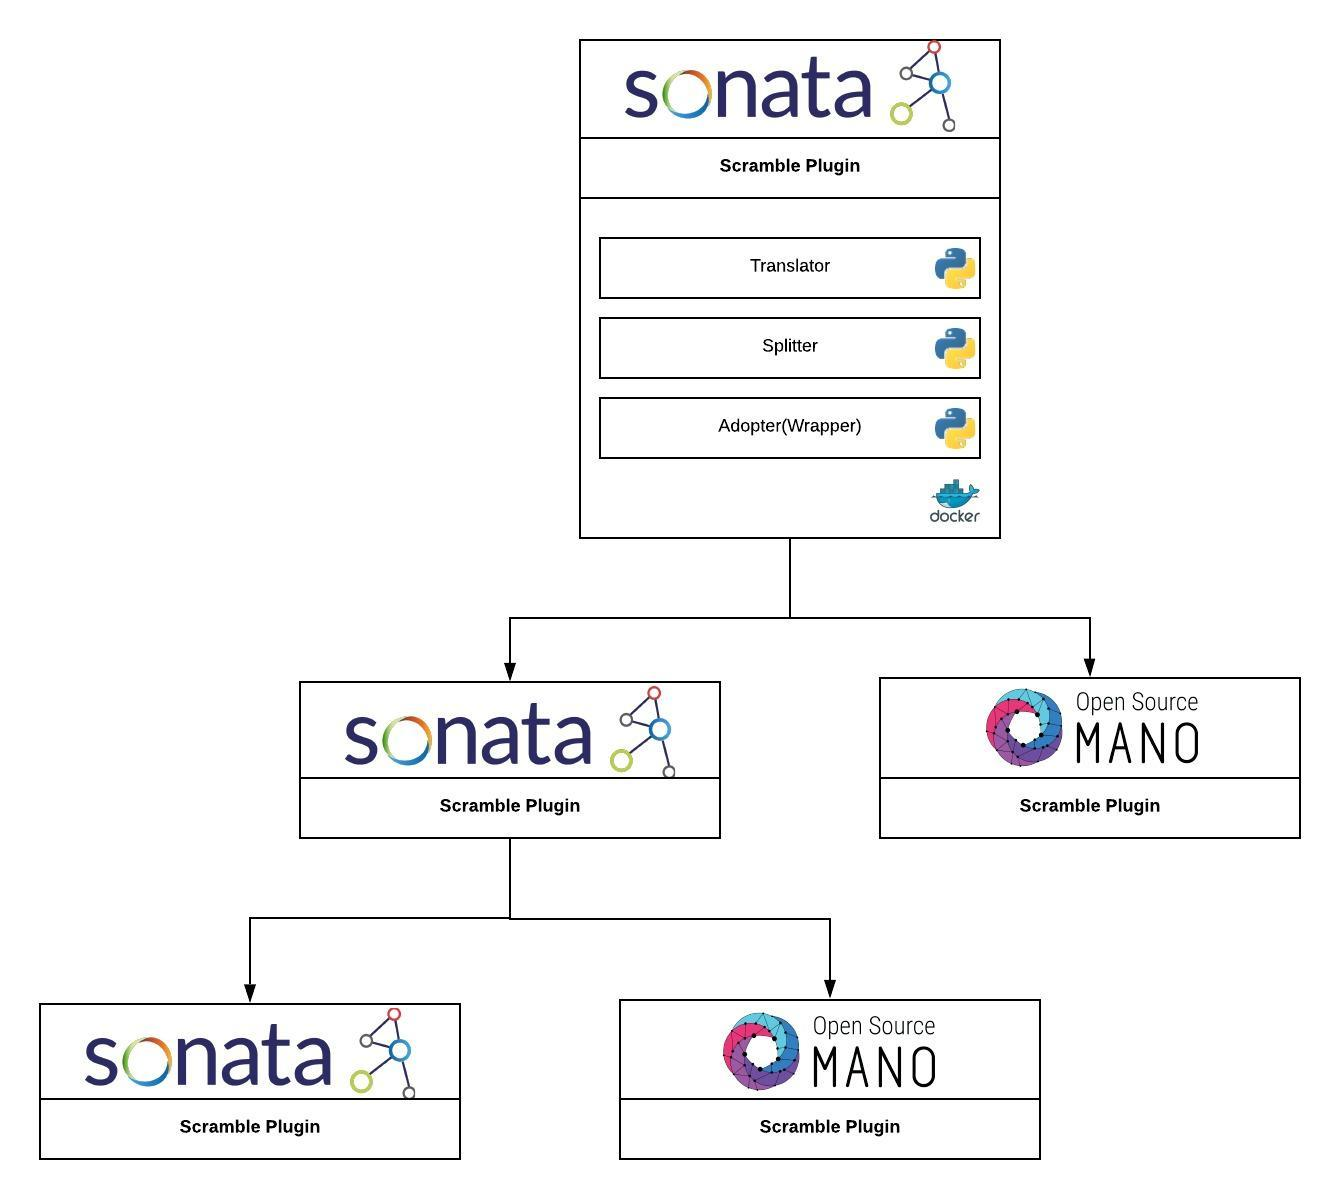
\includegraphics[width=1\linewidth]{figures/scramblearch}
	\caption{Scramble Architecture}
	\label{fig:scramblearch}
\end{figure}
